\documentclass[11pt,class=report,crop=false]{standalone}
\usepackage[screen]{../mathgame}


\begin{document}


%====================================================================
\chapitre{Pixels}
%====================================================================


\insertvideo{oDLcQuFOWRA}{partie 9.1. Pixels}

\insertvideo{TFSAi9Ik-KM}{partie 9.2. Tracé d'un segment - Algorithme de Bresenham}

\insertvideo{uJIw-2pnx0E}{partie 9.3. Anticrénelage}

\insertvideo{1oJdOlUeCmE}{partie 9.4. Tracé d'un cercle}

\insertvideo{GP38pARmO9w}{partie 9.5. Colorier}

\insertvideo{YmIPcqXAcPo}{partie 9.6. Animation 2D}


\objectifs{Comment tracer, pixel par pixel, les figures géométriques de base ?}

%%%%%%%%%%%%%%%%%%%%%%%%%%%%%%%%%%%%%%%%%%%%%%%%%%%%%%%%%%%%%%%%%%%%%
\section{Pixels}

\index{pixel}

%--------------------------------------------------------------------
\subsection{L'unité d'affichage}

Le \defi{pixel} est l'unité élémentaire d'affichage graphique numérique.
Son abréviation est \og{}px\fg{}. Le plus souvent le pixel est assimilé à un carré (ce sera le cas dans ce cours), mais peut aussi parfois être un rectangle.

\myfigure{0.7}{
	\tikzinput{fig-pixels-01}
}

Un pixel peut être noir ou blanc, mais aussi en couleur (le plus souvent obtenue par l'addition des couleurs de trois sous-pixels : un rouge, un vert, un bleu).
La taille d'un pixel est généralement inférieure à \SI{1}{mm}, elle dépend du type d'écran.
Plus la taille d'un pixel est petite, plus la résolution est bonne.
Une autre unité de mesure de la résolution est le \defi{nombre de pixels par pouce}, abrégé par  \og{}ppp\fg{} (ou \emph{ppi} pour \emph{pixels per inch}).
Comme son nom l'indique, il s'agit de compter combien de pixels on peut juxtaposer sur une longueur d'un pouce (1 pouce = \SI{25.4}{mm}).
L'équivalent dans le monde de l'impression est le \emph{dpi} (\emph{dots per inch}).

Voici quelques exemples approximatifs :

\begin{center}
\begin{tabular}{lcc}
Type d'écran & Taille du pixel (mm) & Résolution (ppp) \\
\hline 
Télévision & 0.5 & 50 \\
Ordinateur portable & 0.17 & 150 \\ 
Téléphone & 0.05 & 500 \\
\end{tabular}
\end{center}

L'\oe il humain a une acuité d'environ 1 minute d'arc (c'est-à-dire $1/60$ de degré,  soit $\theta = \frac1{60}\frac{2\pi}{360} \simeq 0.00029$ radian).
Ainsi à une distance $d$, l'\oe il distingue des pixels d'une taille 
$\ell \simeq d \theta$ (avec $\ell$ et $d$ en mètre et $\theta$ en radian).

\myfigure{1.5}{
	\tikzinput{fig-pixels-02}
}

Ainsi en regardant un écran à 20 cm de distance, augmenter la résolution au-delà de 400 ppp ne permet de ressentir une amélioration.
Il faut alors mieux concentrer ses efforts sur la qualité de l'image (vitesse de rafraîchissement, couleurs, rayonnements\ldots) et sur l'énergie (consommation, 
encre électronique\ldots).

\bigskip

\textbf{Un pixel n'est pas vraiment un petit carré !}
Dans ce cours nous assimilerons un pixel à un (petit) carré.
Cependant la réalité est plus compliquée.
Un écran est composé d'une grille de sources lumineuses, appelées des \emph{sous-pixels}. Chaque source illumine une petite zone qui n'est pas nécessairement un carré (cela peut être un disque ou un rectangle). Chaque source est souvent d'une seule couleur parmi rouge/vert/bleu, mais son intensité peut varier. Il n'y a donc physiquement aucun carré dans ce processus !
Sur la photo ci-dessous on pourrait regrouper trois sous-pixels superposés et appeler le petit carré correspondant un pixel, en lui attribuant la couleur résultant des trois sous-pixels.
Il est plus juste de dire que les pixels sont un échantillonnage (relevé en des points d'une grille) du signal lumineux produit par l'écran.

\begin{center}
	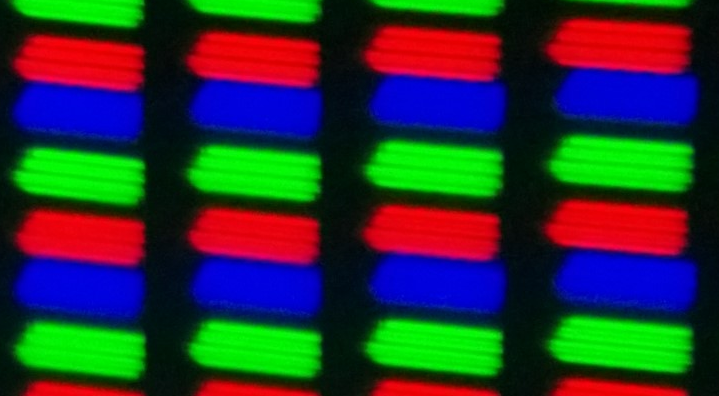
\includegraphics[scale=\myscale,scale=0.25]{figures/sous-pixels}
	
	Les sous-pixels d'un écran de téléphone portable (photo \emph{Wikimedia}).
\end{center}

%--------------------------------------------------------------------
\subsection{Écran}

La \defi{taille} d'un écran est le couple (largeur, hauteur) exprimé en pixels, habituellement notée sous la forme largeur $\times$ hauteur. Le résultat du produit
correspond au nombre total de pixels de l'écran.

\myfigure{0.8}{
	\tikzinput{fig-pixels-03}
}



Le \defi{rapport d'image} est le quotient de la largeur par la hauteur :
$$\text{rapport d'image} = \frac{\text{largeur}}{\text{hauteur}}.$$

Par exemple, pour un écran de taille $1024 \times 768$, cela signifie que chaque ligne contient $1\,024$ pixels et que chaque colonne contient $728$ pixels. Le rapport d'image est
$$r = \frac{1024}{768} = \frac{4}{3} \simeq 1.33.$$

\begin{center}
\begin{tabular}{|l|c|c|c|c|} 
	\hline
	Nom du format & largeur & hauteur & rapport (fraction) & ratio (approché) \\ \hline \hline
	VGA & $640$ & $480$ & $4/3$ &  1.33 \\ \hline	
	HD720 & 1280 & 720 & $16/9$ & 1.77 \\ \hline 
	HD1080 & 1920 & 1080 & $16/9$ & 1.77 \\ \hline 	
	WUXGA & 1920 & $1200$ & $16/10$ & 1.60 \\ \hline 
	4K    & 3840 & 2160 & $16/9$ & 1.77 \\ \hline
	8K    & 7680 & 4320 & $16/9$ & 1.77 \\ \hline
	Image format Cinémascope & $1024$ & $430$ & & 2.38 \\ \hline  
\end{tabular}
\end{center}

\medskip

Le repère des pixels sur un écran a son axe des \og{}$y$\fg{} dirigé vers le bas, contrairement à l'usage en mathématiques (que l'on suivra dans cet ouvrage).
Ainsi le pixel en haut à gauche a pour coordonnées $(0,0)$.

\myfigure{0.8}{
	\tikzinput{fig-pixels-04}
}


%%%%%%%%%%%%%%%%%%%%%%%%%%%%%%%%%%%%%%%%%%%%%%%%%%%%%%%%%%%%%%%%%%%%%
\section{Tracé de droites et de cercles}

%--------------------------------------------------------------------
\subsection{Tracé élémentaire d'un segment}

Le but est de tracer un segment composé de pixels entre deux points $P_1(x_1,y_1)$ et $P_2(x_2,y_2)$. Nous supposons que ces points ont des coordonnées entières ($x_1, y_1, x_2, y_2 \in \Zz$) et qu'un pixel est un carré de côté 
$1$ centré en un couple d'entier $(i,j)$.

\myfigure{0.7}{
	\tikzinput{fig-segment-03}
	\qquad
	\tikzinput{fig-segment-04}
}

L'idée naturelle est de calculer une équation de la droite $(P_1P_2)$. Une équation réduite est $y = \alpha x + \beta$ où $\alpha$ est la pente et $\beta$ l'ordonnée à l'origine.
On va préférer écrire l'équation sous la forme :
$$y = \alpha (x-x_1) + y_1$$
où $(x_1,y_1)$ est un point de la droite et la pente se calcule par 
$\alpha = \frac{\Delta y}{\Delta x} = \frac{y_2-y_1}{x_2-x_1}.$

\myfigure{1}{
	\tikzinput{fig-segment-02}
}
\textbf{Hypothèse.} On suppose $x_1 < x_2$,  $y_1 < y_2$ et $\alpha = \frac{\Delta y}{\Delta x} \le 1$.

Autrement dit, on trace un segment ayant une pente comprise entre $0$ et $1$, c'est-à-dire l'angle formé entre une horizontale et le segment est compris entre \ang{0} et \ang{45}.
Les autres situations s'obtiennent par symétrie et ne seront pas détaillées ici.

Les pixels à colorier ont pour abscisses successives $i=x_1, x_1+1,\ldots,x_2$.
L'ordonnée réelle correspondant à l'abscisse $i$ est $y = \alpha (i-x_1) + y_1$ mais nous voulons une coordonnée entière qui s'obtient par un arrondi :
\mybox{$j = \operatorname{arrondi}(\alpha (i-x_1) + y_1)$}

Remarque :
si $\lfloor x \rfloor$ désigne la partie entière d'un réel $x$ (obtenue par une commande \ci{floor(x)} en \Python{} par exemple) alors :
$$\operatorname{arrondi}(x) = \lfloor x + \tfrac12 \rfloor$$


Pour minimiser les opérations on remarque que lorsque l'on passe de l'abscisse $x$ à l'abscisse $x+1$ alors l'ordonnée passe de $y$ à $y + \alpha$.

\myfigure{0.8}{
	\tikzinput{fig-segment-05}
}

\begin{algorithme}[Algorithme du tracé élémentaire]

\textbf{Entrée :} des entiers $x_1, y_1, x_2, y_2$ vérifiant l'hypothèse.

\textbf{Sortie :} le tracé des pixels reliant $(x_1,y_1)$ à $(x_2,y_2)$.

\begin{itemize}
	\item Calculer $\alpha =  \frac{y_2-y_1}{x_2-x_1}$.
	\item Poser $i = x_1$.
	\item Poser $y = y_1$.
	
	\item Tant que $i \le x_2$ :
	\begin{itemize}
		\item $j = \operatorname{arrondi}(y)$
		\item afficher le pixel $(i,j)$
		\item $i = i + 1$
		\item $y = y + \alpha$
	\end{itemize}
\end{itemize}
\end{algorithme}

\begin{exemple}	
On souhaite tracer le segment reliant $P_1(0,0)$ et $P_2(8,3)$.
On calcule :
$$\alpha =\frac{\Delta y}{\Delta x} = \frac{y_2-y_1}{x_2-x_1} = \frac38 = 0.375.$$

Voici les valeurs lorsqu'on applique l'algorithme :
$$\begin{array}{ccc}
i & y 		& j \\ \hline	
0 & 0       & 0 \\
1 & 0.375   & 0 \\
2 & 0.75    & 1 \\
3 & 1.125   & 1 \\
4 & 1.5     & 2 \\
5 & 1.875   & 2 \\
6 & 2.25    & 2 \\
7 & 2.625   & 3 \\
8 & 3.0     & 3 \\
\end{array}
$$
Ce qui donne :
\myfigure{0.8}{
	\tikzinput{fig-segment-06}
}	
\end{exemple}

Noter que les calculs se font avec des nombres réels et sont donc assez lents.
%D'autres tracés seront vus dans la section suivante.

 

%--------------------------------------------------------------------
\subsection{Algorithme de Bresenham}

\index{algorithme!de Bresenham}

Objectif : trouver un algorithme plus rapide que l'algorithme élémentaire en ne faisant que des calculs sur des entiers. Le résultat est équivalent à l'algorithme précédent mais beaucoup plus rapide.

Voici quelques tracés.

\myfigure{0.6}{
	\tikzinput{fig-segment-07a} 
	\qquad
	\tikzinput{fig-segment-07b}	
}

\myfigure{0.6}{
	\tikzinput{fig-segment-07c}	
}

\begin{algorithme}[Algorithme de Bresenham]

\textbf{Entrée :} des entiers $x_1, y_1, x_2, y_2$ vérifiant l'hypothèse.

\textbf{Sortie :} le tracé des pixels reliant $(x_1,y_1)$ à $(x_2,y_2)$.

\begin{itemize}
	\item Calculer $p = 2\Delta y = 2(y_2-y_1)$.
	\item Calculer $m = 2\Delta y - 2 \Delta x = 2(y_2-y_1) -2(x_2-x_1)$.
	\item Poser $d = 2\Delta y - \Delta x = 2(y_2-y_1) - (x_2-x_1)$.
	
	\item Poser $i = x_1$ et $j = y_1$.
	
	\item Tant que $i \le x_2$ :
	\begin{itemize}
		\item afficher le pixel $(i,j)$
		
		\item 
		si $d < 0$:
		    \begin{itemize}
			\item $d = d+p$
			\end{itemize}
		\item sinon:
		    \begin{itemize}		
			\item $j=j+1$ 
			\item $d=d+m$	
			\end{itemize}					
		\item $i = i + 1$
	\end{itemize}
\end{itemize}
\end{algorithme}

Noter que $p$, $m$ sont des constantes entières avec $p>0$ et $m<0$ ; $d$ est le \og{}défaut\fg{}, c'est une variable qui détermine s'il faut prendre le pixel juste à côté ou bien s'il faut monter d'un cran. Le défaut est alors mis à jour en lui ajoutant selon le cas une valeur fixe $p>0$ ou $m<0$ (si $d < 0$, le nouveau défaut $d+p$ a augmenté ; si $d \ge 0$, le nouveau défaut $d+m$ a diminué car $m<0$).

\myfigure{0.8}{
	\tikzinput{fig-segment-08a}\qquad\qquad\qquad
	\tikzinput{fig-segment-08b}	
}

Noter qu'en plus les opérations sur les entiers sont élémentaires : ce sont des additions et un test de positivité.
% et aussi des multiplications par $2$ qui pour un ordinateur est une opération rapide (car en écriture binaire une multiplication par $2$ c'est juste l'ajout d'un $0$ à droite de l'écriture binaire, de même qu'en écriture décimale la multiplication par $10$ est facile).

\begin{exemple}	

On souhaite tracer le segment reliant $P_1(0,0)$ et $P_2(8,5)$.
On calcule :
$$p=10 \qquad  m=-6 \qquad d_0=2$$

Voici les valeurs lorsqu'on applique l'algorithme :
$$\begin{array}{ccccc}
i & j & d   &  \text{monter ?}		& \begin{array}{c}\text{nouvelle}\\ \text{ valeur de } d \end{array} \\ \hline
0 & 0 & 2   & \text{oui} & -4 \\
1 & 1 & -4  & \text{non} &  6 \\
2 & 1 & 6   & \text{oui} & 0 \\
3 & 2 & 0   & \text{oui} & -6 \\
4 & 3 & -6  & \text{non} &  4 \\
5 & 3 & 4   & \text{oui} & -2 \\
6 & 4 & -2  & \text{non} &  8 \\
7 & 4 & 8   & \text{oui} & 2 \\
8 & 5 &     &     &  \\	
\end{array}
$$
	
\myfigure{0.8}{
	\tikzinput{fig-segment-09}	
}

\end{exemple}


\bigskip
\textbf{Preuve.}
Justifions que l'algorithme est correct.
\begin{itemize}
	\item \textbf{Équation de la droite à coefficients entiers.}
	Nous avons vu qu'une équation de la droite $(P_1P_2)$ est $y = \frac{\Delta y}{\Delta x} (x-x_1) + y_1$ avec $\Delta x =  x_2-x_1$ et $\Delta y = y_2 - y_1$. En multipliant cette équation par l'entier $\Delta x$ on obtient l'équation :
	$$(\Delta y) x - (\Delta x)y - (\Delta y)x_1 + (\Delta x) y_1 = 0$$
	c'est-à-dire une équation $ax+by+c=0$ avec $a,b,c$ qui sont tous les trois des entiers.
	
	Ainsi on définit la fonction :
	$$E(x,y)=ax+by+c$$
	où
	$a=\Delta y$, $b=-\Delta x$, $c=-(\Delta y)x_1 + (\Delta x) y_1 $.
	Cette fonction détermine l'\emph{écart} du point $(x,y)$ par rapport à la droite $(P_1P_2)$ :
	\begin{itemize}
		\item si $E(x,y)=0$, le point $(x,y)$ appartient à la droite,
		\item si $E(x,y)<0$, le point $(x,y)$ est situé au-dessus de la droite,		
		\item si $E(x,y)>0$, le point $(x,y)$ est situé en-dessous de la droite.
	\end{itemize}


	\item \textbf{Monter ou pas ?}
	Centrons en $P(x_k,y_k)$ un pixel déjà correctement colorié. Quels choix avons-nous pour colorier le pixel suivant ? Dans tous les cas le pixel suivant sera sur la colonne d'abscisse $x_k+1$. Mais son ordonnée sera soit $y_k+1$ (point $A$), soit $y_k$ (point $B$).
	
	\medskip

\myfigure{0.8}{
	\tikzinput{fig-segment-10a}\qquad\qquad\qquad
	\tikzinput{fig-segment-10b}	
}
	

	Nous allons utiliser notre fonction d'écart $E$. Noter que l'on a toujours $E(A) \le 0$ et $E(B) > 0$. 	
	On choisit entre $A$ et $B$ celui qui est le plus proche de la droite réelle, c'est-à-dire celui qui a le plus petit écart $|E(A)|$ ou $|E(B)|$ (en valeur absolue).
	Pour savoir lequel choisir on définit le \emph{défaut} par 
	$$D(P) = E(A)+E(B).$$
	
	On retient :
	
	\mycenterline{Si $D(P) \le 0$ alors on choisit $B$, si $D(P)>0$ alors on choisit $A$.}
	
	En effet, si $D(P) \le 0$ alors $E(A)+E(B) \le 0$ donc $E(B) \le -E(A)$ mais comme $E(A)\le0$ et $E(B)>0$ alors on a bien $|E(B)| \le |E(A)|$.

	
	\item \textbf{Calcul du défaut.}
	Calculons $D_k$ le défaut au point $P(x_k,y_k)$ :
    \begin{align*}
	D_k 
	&= D(x_k,y_k) = E(A) + E(B) = E(x_k+1,y_k+1)+E(x_k+1,y_k) \\
	&= a (x_k+1) +b(y_k+1) + c \quad + \quad a (x_k+1) +by_k + c  \\
	&= 2a x_k +2b y_k + 2a+b+2c
   \end{align*}	
	
	En particulier $D_0$ le défaut au point initial $(x_1,y_1)$ est :
	\begin{align*}
	D_0 
	  &= 2a x_1 +2b y_1 + 2a+b+2c \\
	  &= 2(ax_1+by_1+c) + 2a+b   \qquad (\star)\\
	  &= 2a + b  \\
	  &= 2\Delta y - \Delta x 
	\end{align*}
	
	À la ligne $(\star)$ on a utilisé le fait que le point initial $(x_1,y_1)$ est exactement sur la droite, donc $ax_1+by_1+c=0$.
		
	\item \textbf{Formule de récurrence du défaut.}
	
	Nous allons maintenant trouver la relation qui lie le défaut d'un pixel $D_k$ au défaut du pixel suivant $D_{k+1}$.
	On part toujours du point $P(x_k,y_k)$, on a déjà calculé $D_k$. Le calcul de $D_{k+1}$ dépend du choix $A$ ou $B$ pour le pixel d'abscisse $x_{k+1}$.
	
	\myfigure{0.7}{
		\tikzinput{fig-segment-11a}\qquad\qquad\qquad
		\tikzinput{fig-segment-11b}	
	}
	
	\textbf{Cas du choix $A$ (cas $D_k\ge0$)}.
	Le pixel suivant a pour abscisse $x_k+2$ et pour ordonnée soit $y_k+2$ ($A'$), soit $y_k+1$ ($B'$).
	

	\myfigure{0.8}{
	\tikzinput{fig-segment-12a}
    }

	
	Calculons alors le défaut :
	\begin{align*}
		D_{k+1} 
		&= E(A') + E(B') = E(x_k+2,y_k+2)+E(x_k+2,y_k+1) \\
		&= a (x_k+2) +b(y_k+2) + c \quad + \quad a (x_k+2) +b(y_k+1) + c  \\
		&= 2a x_k + 2by_k + 4a+3b+2c\\
		&= D_k + 2a+2b
	\end{align*}
	Ainsi en posant $m = 2a+2b = 2\Delta y - 2 \Delta x$, on obtient la formule de récurrence :
	$$D_{k+1} = D_k + m.$$
	
	
	\textbf{Cas du choix $B$ (cas $D_k<0$)}.	
	Le pixel suivant a pour abscisse $x_k+2$ et pour ordonnée soit $y_k+1$ ($A'$), soit $y_k$ ($B'$).

	\myfigure{0.8}{
	\tikzinput{fig-segment-12b}
    }

	Calculons alors le défaut :
	\begin{align*}
		D_{k+1} 
		&= E(A') + E(B') = E(x_k+2,y_k+1)+E(x_k+2,y_k) \\
		&= a (x_k+2) +b(y_k+1) + c \quad + \quad a (x_k+2) +by_k + c  \\
		&= 2a x_k + 2by_k + 4a+b+2c\\
		&= D_k + 2a
	\end{align*}
	Ainsi en posant $p = 2a = 2\Delta y$, on obtient la formule de récurrence :
	$$D_{k+1} = D_k + p.$$
	
	Conclusion : on sait calculer $D_{k+1}$ qui permet de choisir entre $A'$ et $B'$.
	Ainsi à partir de $D_0$ et par les formules de récurrence ci-dessus on calcule la suite des défauts $D_{k}$ et on sait donc s'il faut monter le pixel d'un cran ou pas.
		
\end{itemize}



%--------------------------------------------------------------------
\subsection{Anticrénelage (\emph{antialiasing})}

\index{anticrenelage@anticrénelage/\emph{antialiasing}}

Le tracé d'un segment est nécessairement une approximation d'un tracé de droite, qui présente des défauts de visualisation appelée \og{}crénelage\fg{}. On remédie à cette imperfection à l'aide d'un 
anticrénelage (\emph{antialiasing}) qui colorie aussi le pixel laissé de côté (le pixel $A$ ou $B$ écarté dans les algorithmes précédents).

\myfigure{0.7}{
	\tikzinput{fig-antialiasing-01a}\qquad\qquad
	\tikzinput{fig-antialiasing-01b}	
}


\myfigure{0.2}{
	\tikzinput{fig-antialiasing-02a}\qquad\qquad\qquad
	\tikzinput{fig-antialiasing-02b}	
}

\myfigure{0.05}{
	\tikzinput{fig-antialiasing-02a}\qquad\qquad\qquad
	\tikzinput{fig-antialiasing-02b}	
}


De près le rendu n'est pas impressionnant mais de loin l'amélioration est sensible.

Nous allons expliquer un algorithme simple pour dessiner un segment avec anticrénelage. 
Nous avons donc deux pixels l'un au-dessus de l'autre à colorier : le pixel $A$ et le pixel $B$.
Comment répartir 100\% de couleur  entre ces deux pixels ?

Commençons par expliquer une analogie issue de la physique.
Considérons deux masses ponctuelles liées entre elles : $m_A$ centrée en $A$ et $m_B$ centrée en $B$. Lorsque l'on regarde ce système d'assez loin on peut le considérer comme un système formé d'une seule masse ponctuelle : la masse totale est $m=m_A+m_B$ et est centrée au centre de gravité $G$. Ce centre de gravité $G$ est défini par la relation :
$$\ell_A m_A = \ell_B m_B$$
où $\ell_A = AG$ et $\ell_B = BG$.

\myfigure{1}{
	\tikzinput{fig-antialiasing-03}	
}

\myfigure{1}{
	\tikzinput{fig-antialiasing-04}	
}

Reprenons cette idée : nous répartissons une masse totale $m=1$ (100\% de la couleur) centrée exactement sur la droite réelle en $G$ entre deux points $A$ et $B$.

Notons $(x,y)$ le point $G$ de la droite réelle. Soit alors :
$$j = \lfloor y \rfloor \qquad \text{ et } \qquad \ell = y - \lfloor y \rfloor$$
respectivement la partie entière et la partie fractionnaire de $y$.
La distance $BG$ est $\ell$ et la distance $AG$ est $1-\ell$ (car $AB = 1$).
Ainsi pour que les couleurs satisfassent la formule du centre de gravité il faut choisir 
$m_A = \ell$ et $m_B = 1-\ell$ comme intensité de couleur respectivement pour $A$ et $B$ car on a alors bien
$(1-\ell) \ell = \ell (1-\ell)$.

On adapte l'algorithme du tracé élémentaire pour y ajouter l'anticrénelage.

\begin{algorithme}[Algorithme d'anticrénelage]

\textbf{Entrée :} des entiers $x_1, y_1, x_2, y_2$ vérifiant l'hypothèse.

\textbf{Sortie :} le tracé des pixels reliant $(x_1,y_1)$ à $(x_2,y_2)$.

\begin{itemize}
	\item Calculer $\alpha =  \frac{y_2-y_1}{x_2-x_1}$.
	\item Poser $i = x_1$.
	\item Poser $y = y_1$.
	
	\item Tant que $i \le x_2$ :
	\begin{itemize}
		\item $j = \lfloor y \rfloor$
		\item $\ell = y - \lfloor y \rfloor$
		\item afficher le pixel $(i,j)$ avec l'intensité de couleur $1-\ell$
		\item afficher le pixel $(i,j+1)$ avec l'intensité de couleur $\ell$		
		\item $i = i + 1$
		\item $y = y + \alpha$
	\end{itemize}
\end{itemize}
\end{algorithme}


%--------------------------------------------------------------------
\subsection{Tracé d'un cercle}

On souhaite tracer un cercle de rayon $r$ centré en $(x_0,y_0)$.
Ce cercle a pour équation :
$$(x-x_0)^2 + (y-y_0)^2 = r^2.$$

Pour cela on va se contenter de tracer l'arc de cercle compris entre \ang{90} et \ang{45}. Le reste s'obtiendra par symétrie.


\myfigure{0.5}{
	\tikzinput{fig-cercle-01}	
}

Voici quelques exemples.

\myfigure{0.4}{
	\tikzinput{fig-cercle-02a}\qquad	
	\tikzinput{fig-cercle-02b}\qquad
	\tikzinput{fig-cercle-02c}\qquad		
}

\begin{center}
\begin{minipage}{0.45\textwidth}	
\myfigure{0.25}{
	\tikzinput{fig-cercle-02d}		
}
\end{minipage}
\begin{minipage}{0.45\textwidth}
\myfigure{0.1}{
	\tikzinput{fig-cercle-02e}		
}
\end{minipage}
\end{center}
Voici l'algorithme du tracé de l'arc de cercle de type Bresenham car il n'utilise que des entiers. Le point de départ est le point $(0,r)$ (point le plus haut du cercle).

\begin{algorithme}[Algorithme de tracé de cercle]

\textbf{Entrée :} des entiers $x_0, y_0$ pour le centre et un entier $r$ pour le rayon.

\textbf{Sortie :} le tracé d'un arc du cercle centré en $(x_0,y_0)$ de rayon $r$.

\begin{itemize}
	\item Poser $i = 0$.
    \item Poser $j = r$.	
	\item Poser $d = 3 - 2r$.
		
	\item Tant que $i \le j$ :
	\begin{itemize}
		\item afficher le pixel $(x_0+i,y_0+j)$
		
		\item si $d < 0$ :
			\begin{itemize}
			\item $d = d+ 4i+6$
			\end{itemize}
		\item sinon:
			\begin{itemize}		
			\item $d=d+4i-4j+10$		
			\item $j=j-1$
			\end{itemize}			
		\item $i = i + 1$
	\end{itemize}
\end{itemize}
\end{algorithme}
	
Sur la portion tracée (de $\ang{90}$ à $\ang{45}$) il y a exactement un pixel pour chaque $i$. Pour obtenir le cercle complet, en plus du pixel en $(x_0+i,y_0+j)$, il faut afficher par symétrie les pixels en 
$(x_0+j,y_0+i)$, $(x_0-i,y_0+j)$, $(x_0-j,y_0+i)$
$(x_0+i,y_0-j)$, $(x_0+j,y_0-i)$, $(x_0-i,y_0-j)$, $(x_0-j,y_0-i)$.


\textbf{Preuve.}
La preuve est similaire à celle de l'algorithme du tracé d'un segment de Bresenham.

\begin{itemize}
	\item \textbf{Équation du cercle.}
	
On suppose que le cercle est centré à l'origine : $(x_0,y_0)=(0,0)$. Un cercle quelconque s'obtiendrait par translation.
Soit la fonction d'écart :
$$E(x,y) = x^2 + y^2 -r^2$$
Si $E(x,y)=0$ le point $(x,y)$ est sur le cercle, si $E(x,y)>0$ le point est à l'extérieur, si $E(x,y)<0$ le point est à l'intérieur.

\myfigure{0.5}{
	\tikzinput{fig-cercle-03}	
}

	\item \textbf{Descendre ou pas ?}

Pour un pixel centré en $P$ déjà tracé, nous devons choisir pour le pixel suivant entre $A$ et $B$. 
On choisit le point le plus proche du cercle, c'est-à-dire le minimum entre 
$|E(A)|$ ou $|E(B)|$.
On définit le \emph{défaut} par 
$$D(P) = E(A)+E(B)$$ 
et on a :
\mycenterline{Si $D(P) < 0$ alors on choisit $A$, si $D(P) \ge 0$ alors on choisit $B$.}

\medskip

\myfigure{0.8}{
	\tikzinput{fig-cercle-04a}\qquad\qquad\qquad
	\tikzinput{fig-cercle-04b}	
}

\item \textbf{Calcul du défaut.}
Calculons $D_k$ le défaut au point $P(x_k,y_k)$ :
\begin{align*}
	D_k 
	&= D(x_k,y_k) = E(A) + E(B) = E(x_k+1,y_k)+E(x_k+1,y_k-1) \\
	&= (x_k + 1)^2 + y_k^2-r^2 \quad + \quad  (x_k + 1)^2 + (y_k-1)^2-r^2\\
	&= 2x_k^2 +2y_k^2 + 4x_k - 2y_k + 3 -2r^2
\end{align*}	

En particulier $D_0$ le défaut au point initial $(0,r)$ vaut :
$$D_0 = 3 - 2r.$$


\item \textbf{Formule de récurrence du défaut.}

On part du point $P(x_k,y_k)$, connaissant $D_k$ on calcule $D_{k+1}$ en fonction du choix $A$ ou $B$ pour le pixel d'abscisse $x_{k+1}$.


\myfigure{0.7}{
	\tikzinput{fig-cercle-05a}\qquad\qquad\qquad
	\tikzinput{fig-cercle-05b}	
}


\textbf{Cas du choix $A$ (cas $D_k<0$)}.
Le pixel suivant a pour abscisse $x_k+2$ et pour ordonnée soit $y_k$ ($A'$), soit $y_k-1$ ($B'$).


\myfigure{0.8}{
	\tikzinput{fig-cercle-06a}
}

Le défaut se calcule ainsi :
\begin{align*}
	D_{k+1} 
	&= E(A') + E(B') = E(x_k+2,y_k)+E(x_k+2,y_k-1) \\
	&=  (x_k + 2)^2 + y_k^2-r^2 \quad + \quad  (x_k + 2)^2 + (y_k-1)^2-r^2\\
	&= D_k + 4x_k+6
\end{align*}

\textbf{Cas du choix $B$ (cas $D_k\ge0$)}.	
Le pixel suivant a pour abscisse $x_k+2$ et pour ordonnée soit $y_k-1$ ($A'$), soit $y_k-2$ ($B'$).

\myfigure{0.8}{
	\tikzinput{fig-cercle-06b}
}


\begin{align*}
	D_{k+1} 
	&= E(A') + E(B') = E(x_k+2,y_k-1)+E(x_k+2,y_k-2) \\
	&=  (x_k + 2)^2 + (y_k-1)^2-r^2 \quad + \quad  (x_k + 2)^2 + (y_k-2)^2-r^2\\
	&= D_k + 4x_k-4y_k+10
\end{align*}

Conclusion : on sait calculer $D_{k+1}$ qui permet de choisir entre $A'$ et $B'$.

\end{itemize}



%%%%%%%%%%%%%%%%%%%%%%%%%%%%%%%%%%%%%%%%%%%%%%%%%%%%%%%%%%%%%%%%%%%%%
\section{Colorier}

\index{algorithme!de coloriage}

%--------------------------------------------------------------------
\subsection{Colorier par diffusion}

\textbf{Objectif.} On considère une image formée par exemple de pixels noirs et blancs.
On souhaite colorier en gris une zone de l'image.
Pour cela, on part d'un pixel initial (la graine, \emph{seed}) et il faut colorier en gris toute la zone de pixels blancs contenant la graine et bordée par des pixels noirs.

\myfigure{0.8}{
	\tikzinput{fig-fill-01}
}

%\begin{center}
%	
\includegraphics[scale=\myscale,scale=0.3]{figures/fill01_000}\qquad\qquad
%	
\includegraphics[scale=\myscale,scale=0.3]{figures/fill01_368}
%\end{center}

\textbf{Principe.} On part de la graine, qu'on colorie en gris. Pour chacun de ses quatre pixels voisins (gauche, bas, droite, haut), si c'est un pixel blanc, on applique le processus à partir de ce nouveau pixel.

Ci-dessous la graine et ses quatre voisins.
\begin{center}
	
\includegraphics[scale=\myscale,scale=0.15]{figures/fill01_000}\quad
	
\includegraphics[scale=\myscale,scale=0.15]{figures/fill01_001}\quad
	
\includegraphics[scale=\myscale,scale=0.15]{figures/fill01_002}\quad
    
\includegraphics[scale=\myscale,scale=0.15]{figures/fill01_003}\quad
	
\includegraphics[scale=\myscale,scale=0.15]{figures/fill01_004}\quad
\end{center}

\textbf{Mise en \oe uvre.} Ce procédé peut être traduit en algorithmes par différentes méthodes : algorithme récursif, algorithme avec une pile ou algorithme avec une file. Dans tous les cas ce sont des algorithmes qui utilisent beaucoup de mémoire afin de stocker les pixels en attente d'être traités. 
On choisit un algorithme avec file (\emph{queue} ou \emph{fifo}, \emph{first in, first out}) un peu moins gourmand en mémoire que les autres choix.

\begin{algorithme}[Algorithme de remplissage par diffusion (\emph{flood fill})]

\textbf{Entrée :} un tableau de pixels noirs ou blancs, un pixel initial $(x_0,y_0)$ (la graine)

\textbf{Sortie :} un tableau de pixels noirs, blancs ou gris

\begin{itemize}
	\item \ci{file} $= [ (x_0,y_0)]$

	\item Tant que la \ci{file} n'est pas vide :
	\begin{itemize}
		\item prendre $(x,y)$ un élément de \ci{file} (et le retirer de la file)
		\item si $(x,y)$ est un pixel blanc :
		\begin{itemize}
			\item le colorier en gris,
			\item ajouter à la \ci{file} les quatre voisins $(x-1,y)$, $(x,y+1)$, $(x+1,y)$, $(x,y-1)$.
		\end{itemize}
	\end{itemize}
\end{itemize}
\end{algorithme}


Quelques étapes du processus :	
\begin{center}
	
\includegraphics[scale=\myscale,scale=0.15]{figures/fill01_000}\quad
	
\includegraphics[scale=\myscale,scale=0.15]{figures/fill01_004}\quad
	
\includegraphics[scale=\myscale,scale=0.15]{figures/fill01_015}\quad
	
\includegraphics[scale=\myscale,scale=0.15]{figures/fill01_050}\quad
	
\includegraphics[scale=\myscale,scale=0.15]{figures/fill01_112}\quad
	
\includegraphics[scale=\myscale,scale=0.15]{figures/fill01_368}
\end{center}
	

%--------------------------------------------------------------------
\subsection{Colorier par balayage}


Le coloriage par balayage en un peu plus performant au niveau de la mémoire car il colorie une portion de ligne avant d'ajouter les pixels au-dessus ou en-dessous dans la file d'attente.

\begin{algorithme}[Algorithme de balayage (\emph{scan fill})]

\textbf{Entrée :} un tableau de pixels noirs ou blancs, un pixel initial $(x_0,y_0)$ (la graine)

\textbf{Sortie :} un tableau de pixels noirs, blancs ou gris

\begin{itemize}
	\item \ci{file} $= [ (x_0,y_0)]$
	
	\item Tant que la \ci{file} n'est pas vide :
	\begin{itemize}
		\item prendre $(x,y)$ un élément de \ci{file} (et le retirer de la file)
	
		\item poser $x_{\text{min}} = x-1$
		\item tant que $(x_{\text{min}}, y)$ est un pixel blanc :
		\begin{itemize}
			\item le colorier en gris,
			\item faire $x_{\text{min}} = x_{\text{min}} - 1$.
        \end{itemize}
	
		\item poser $x_{\text{max}} = x$
		\item tant que $(x_{\text{max}}, y)$ est un pixel blanc :
		\begin{itemize}
			\item le colorier en gris,
			\item faire $x_{\text{max}} = x_{\text{max}} + 1$.
        \end{itemize}
	
		\item Pour chaque $x'$ entre $x_{\text{min}}+1$ et $x_{\text{max}}-1$ :
		\begin{itemize}
		    \item si $(x',y+1)$ est un pixel blanc, l'ajouter à la file,
			\item si $(x',y-1)$ est un pixel blanc, l'ajouter à la file.			
        \end{itemize}
		
	\end{itemize}
\end{itemize}
\end{algorithme}
	
Ci-dessous la graine et les premières lignes.
\begin{center}
	
\includegraphics[scale=\myscale,scale=0.20]{figures/fill02_000}\quad
	
\includegraphics[scale=\myscale,scale=0.20]{figures/fill02_001}\quad
	
\includegraphics[scale=\myscale,scale=0.20]{figures/fill02_002}\quad
	
\includegraphics[scale=\myscale,scale=0.20]{figures/fill02_003}
\end{center}

Quelques étapes plus avancées:	
\begin{center}
	
\includegraphics[scale=\myscale,scale=0.20]{figures/fill02_012}\quad
	
\includegraphics[scale=\myscale,scale=0.20]{figures/fill02_054}\quad
	
\includegraphics[scale=\myscale,scale=0.20]{figures/fill02_065}\quad
	
\includegraphics[scale=\myscale,scale=0.20]{figures/fill02_077}
\end{center}

%%%%%%%%%%%%%%%%%%%%%%%%%%%%%%%%%%%%%%%%%%%%%%%%%%%%%%%%%%%%%%%%%%%%%
\section{Animation}

\index{animation}

Nous expliquons quelques principes liés à l'animation des images.
Les premiers dessins animés étaient basés sur des \emph{calques} : une image fixe pour le calque de l'arrière-plan, un calque pour le premier plan avec par exemple un personnage à redessiner de nombreuses fois afin de simuler le mouvement et éventuellement des calques intermédiaires. On retrouvait aussi cette technique au cinéma où certains arrières-plans étaient peints. 


%--------------------------------------------------------------------
\subsection{Perspective atmosphérique}


Voyons comment la technique des calques permet de simuler un paysage.

La \defi{perspective atmosphérique}\index{perspective!atmospherique@atmosphérique} est une façon de représenter l'éloignement des différents plans ou calques par des teintes plus claires, des contrastes moins élevés et des couleurs plus grises (la saturation diminue).

Cela reflète des phénomènes physiques réels, certaines particules de l'atmosphère (molécules d'air, gouttelettes d'eau, fumées\ldots) diffractent la lumière (particulièrement les longueurs d'ondes plus courtes comme le bleu).


\myfigure{0.6}{
	\tikzinput{fig-atmo-01}\qquad
    \tikzinput{fig-atmo-02}
}

Il existe un modèle de couleurs HSV (\emph{Hue/Saturation/Value} : Teinte/Saturation/Luminosité) pour lequel il suffit donc de changer le paramètre de saturation.

Ci-dessous les couleurs obtenues pour $(h,s,b)$ avec $h=0.66$, $b=0.8$ et la saturation $s$ variant de $0$ à $1$.
\myfigure{0.7}{\tikzinput{fig-atmo-03}}

%--------------------------------------------------------------------
\subsection{La 2.5D}

Comme son nom le suggère, la 2.5D est un ensemble des techniques d'animation qui permettent de simuler une scène 3D. C'est le cas de beaucoup de jeux vidéos de stratégie où le point de vue du joueur est au-dessus du plateau de jeu. Les objets représentés en perspective (par exemple ci-dessous les immeubles) sont des petites images 2D pré-dessinées.
C'est une technique efficace mais qui nécessite de fixer ou de limiter fortement le choix de la vue du joueur.
   
\begin{center}
	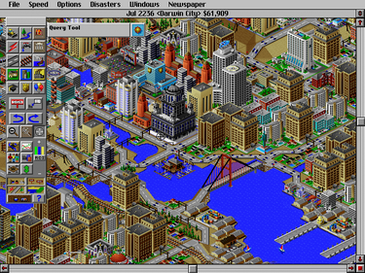
\includegraphics[scale=\myscale,scale=0.6]{figures/simcity}
	
	\emph{SimCity 2000 (images : Wikipedia)}
\end{center}

%--------------------------------------------------------------------
\subsection{Principe de l'animation 2D}

Vous le savez, on simule le mouvement à l'écran par un succession rapide d'images.
Ainsi les pixels ne se déplacent pas, mais seule leur couleur change.
Le cerveau humain, entraîné par les objets réels en mouvement, reconstitue un déplacement à partir d'images fixes.

\myfigure{0.4}{
	\tikzinput{fig-anim-01a}\quad
	\tikzinput{fig-anim-01b}\quad
	\tikzinput{fig-anim-01c}		
}

Pour réaliser de petits jeux animés, les modules de \emph{Pygame} de \Python{} sont très sympas.
On explique ci-dessous les principes de l'animation 2D en suivant la philosophie de \emph{Pygame}.


\textbf{Animation 1D.}

Commençons par une animation très élémentaire en une seule dimension.
Les objets en jeu sont :
\begin{itemize}
	\item \ci{fond} qui est l'image d'arrière-plan représentée ici par une liste de \ci{0},
	\item un entier $p$ qui représente la position d'un personnage, ce personnage est représenté par un \ci{1},
	\item \ci{ecran} qui est l'image finale affichée, et sera donc une juxtaposition de \ci{0} et de \ci{1}.
\end{itemize}

Les étapes de l'animation sont les suivantes :
\begin{itemize}
	\item \emph{Initialisation.}
	On initialise \ci{ecran} avec l'image d'arrière-plan \ci{fond} :
	\mycenterline{\ci{0000000000}}
	On définit une position de départ, par exemple $p=3$.
	
	\item \emph{Affichage.} Par \ci{ecran}$[p] = $\,\ci{1} on affiche le personnage :
	\mycenterline{\ci{0001000000}}	
	
	\item \emph{Déplacement.}
	\begin{itemize}
		\item \emph{Effacer le personnage.} \ci{ecran}$[p] = $\,\ci{0}
		\item \emph{Changer la position.} $p = p+1$.
		\item \emph{Réafficher le personnage.} \ci{ecran}$[p] = $\,\ci{1}		
	\end{itemize}

\end{itemize}

En répétant le déplacement on obtient, successivement :
\mycenterline{\ci{0001000000}}
\mycenterline{\ci{0000100000}}
\mycenterline{\ci{0000010000}}	
\mycenterline{\ci{0000001000}}
\mycenterline{\ci{0000000100}}


\bigskip

\textbf{Animation 2D.}

Le principe est similaire, il nous faut une image de fond, une image à afficher pour l'objet à déplacer.
L'affichage à l'écran correspond à affecter des valeurs à la mémoire graphique (\emph{screen buffer}) ; on représente ici l'écran comme une image.

\myfigure{0.9}{\tikzinput{fig-anim-02}}


L'opération fondamentale est la \emph{copie rapide} ou \emph{blit} (pour \emph{bit-block transfer}) qui consiste à copier les données d'une image dans la mémoire graphique. 
Concrètement cela signifie copier une image et l'afficher à l'écran à une position donnée (figure (a)) ou bien copier seulement une partie d'une image (figure (b)).

\myfigure{0.8}{
	\tikzinput{fig-anim-03a}
}
\myfigure{0.8}{
	\tikzinput{fig-anim-03b}
}


Le second cas de figure nous sert à effacer le personnage avant de le déplacer, plus exactement on copie à l'écran la portion de l'arrière-plan à la place qu'occupait le personnage.

Le processus de l'animation est alors le même que précédemment :
\begin{itemize}
	\item \emph{(a) Initialisation.}
	On initialise \ci{ecran} avec l'image d'arrière-plan \ci{fond} :
	
	\item \emph{(b) Affichage.} On affiche le personnage à une position donnée.
	
	\item \emph{Déplacement.} (À répéter)
	\begin{itemize}
		\item \emph{(c) Effacement du personnage.} Pour cela on copie la portion de l'arrière-plan correspondant à l'emplacement qu'occupe le personnage.
		
		\item \emph{(d) Affichage du personnage à sa nouvelle position.}
	\end{itemize}
	
\end{itemize}

La vitesse du mouvement est contrôlée par la longueur du déplacement et la durée de la pause  entre deux répétitions.

\myfigure{0.6}{
	\tikzinput{fig-anim-05}
}


%\myfigure{0.8}{
%	\tikzinput{fig-anim-04a}
%}
%\myfigure{0.8}{
%	\tikzinput{fig-anim-04b}
%}
%\myfigure{0.8}{
%	\tikzinput{fig-anim-04c}
%}
%\myfigure{0.8}{
%	\tikzinput{fig-anim-04d}
%}

\end{document}
